% ------------------------------------------------------------------------
% -*-TeX-*- -*-Hard-*- Smart Wrapping
% ------------------------------------------------------------------------
\def\baselinestretch{1}

\chapter{Result, Evaluation and Discussion}
\section{Exploratory Analysis Result}
\subsection{Exploratory Analysis }
\subsubsection{Data Distribution}
\begin{figure}[H]
    \centering
    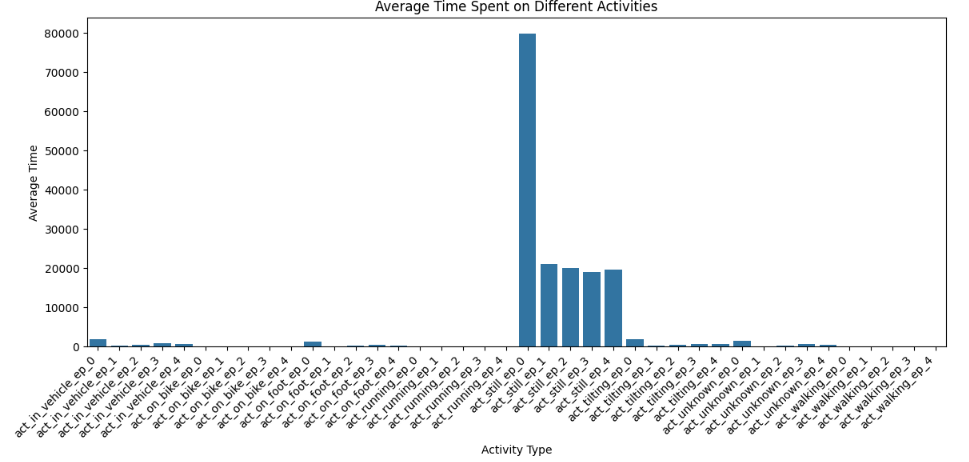
\includegraphics[width=0.5\linewidth]{Dissertation 24/activity.png}
    \caption{Activity Distribution}
    \label{fig:activ}
\end{figure}

\begin{figure}[H]
    \centering
    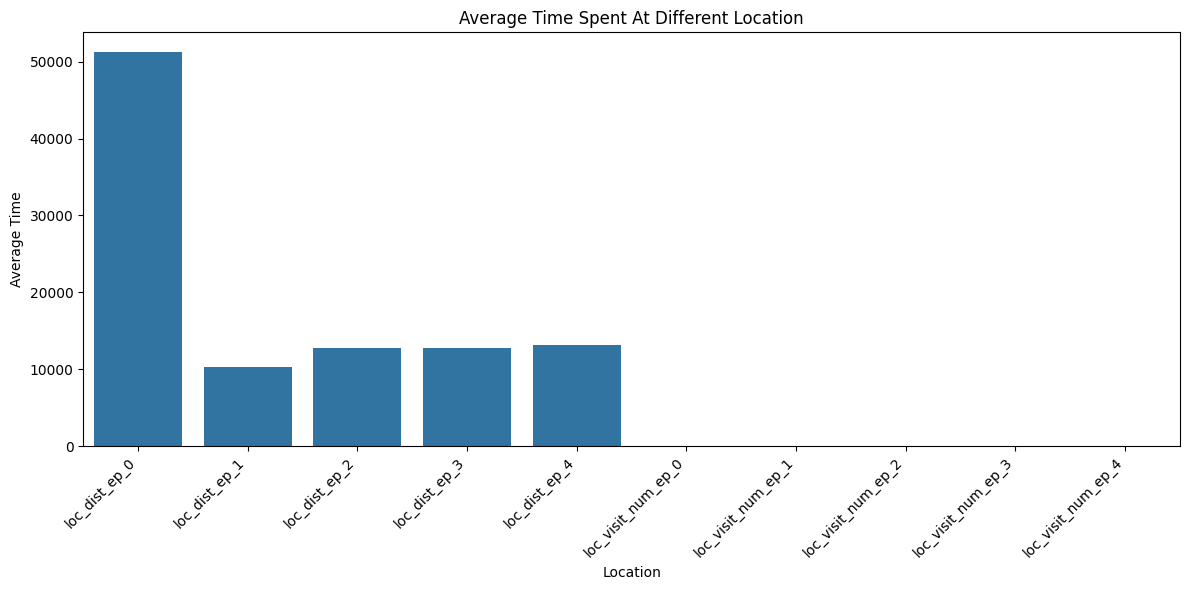
\includegraphics[width=0.5\linewidth]{Dissertation 24/loca.png}
    \caption{Location Distribution}
    \label{fig:loca}
\end{figure}

\begin{figure}[H]
    \centering
    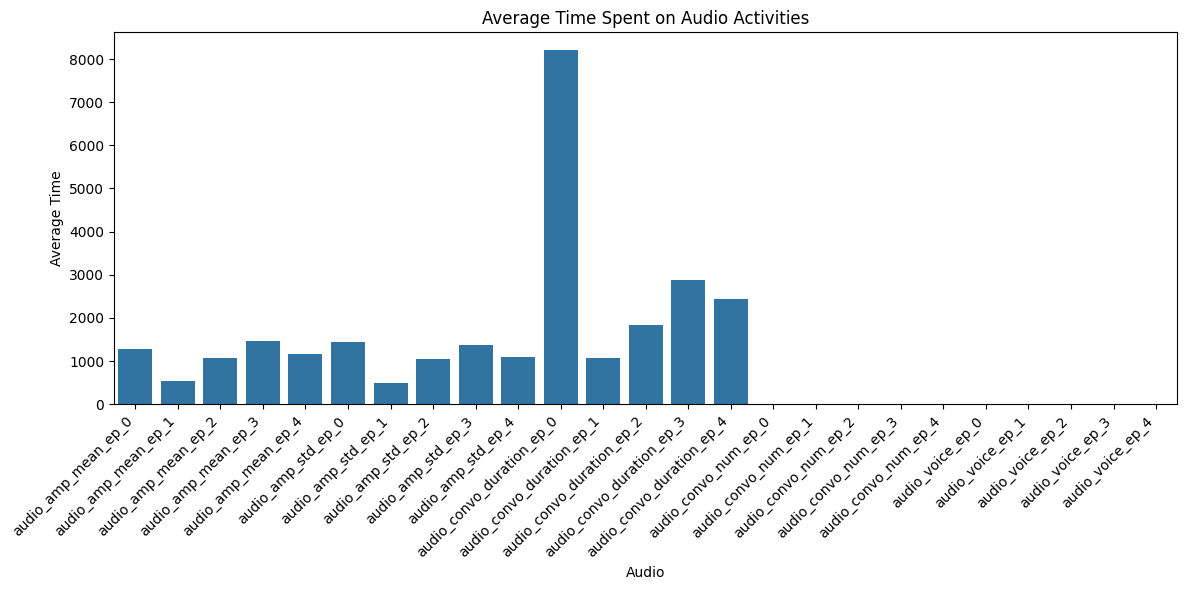
\includegraphics[width=0.5\linewidth]{Dissertation 24/activt.png}
    \caption{Audio Distribution}
    \label{fig:audio}
\end{figure}
From Figures \ref{fig:activ}, \ref{fig:loca} and \ref{fig:audio},  it can be observed that most activities peak during the 12-18 hour period (12 PM to 6 PM) which aligns with typical patterns of increased movement and activity during the day, while The 'still' activity peaks during the 0-6 hour period (12 AM to 6 AM), which aligns with typical sleeping hours. This analysis provides a more accurate representation of activity patterns throughout the day, correctly divided into four 6-hour blocks. It shows clear variations in activity levels across different times of the day, with most physical activities peaking in the afternoon, and stationary activity peaking during the night

\subsubsection{Descriptive Statistics}
\begin{figure}[H]
    \centering
    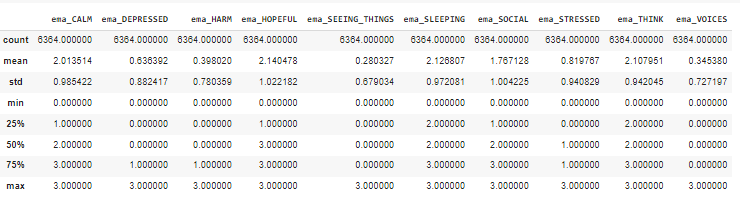
\includegraphics[width=0.5\linewidth]{descript.png}
    \caption{Descriptive Statistics For EMA}
    \label{fig:descr}
\end{figure}

From \ref{fig:descr}, it can be observed that participants generally reported feeling calm (mean = 2.02) and hopeful (mean = 2.14), with moderate variability in these experiences. Depression, self-harm thoughts, and hallucinations were relatively uncommon, though some participants did report higher levels of these issues, as indicated by the higher standard deviations. Overall, the positive EMA score was higher than the negative EMA score, suggesting participants experienced more positive than negative experiences, though there was notable variability in both. 

\subsubsection{Correlation Analysis}
\begin{figure}[H]
    \centering
    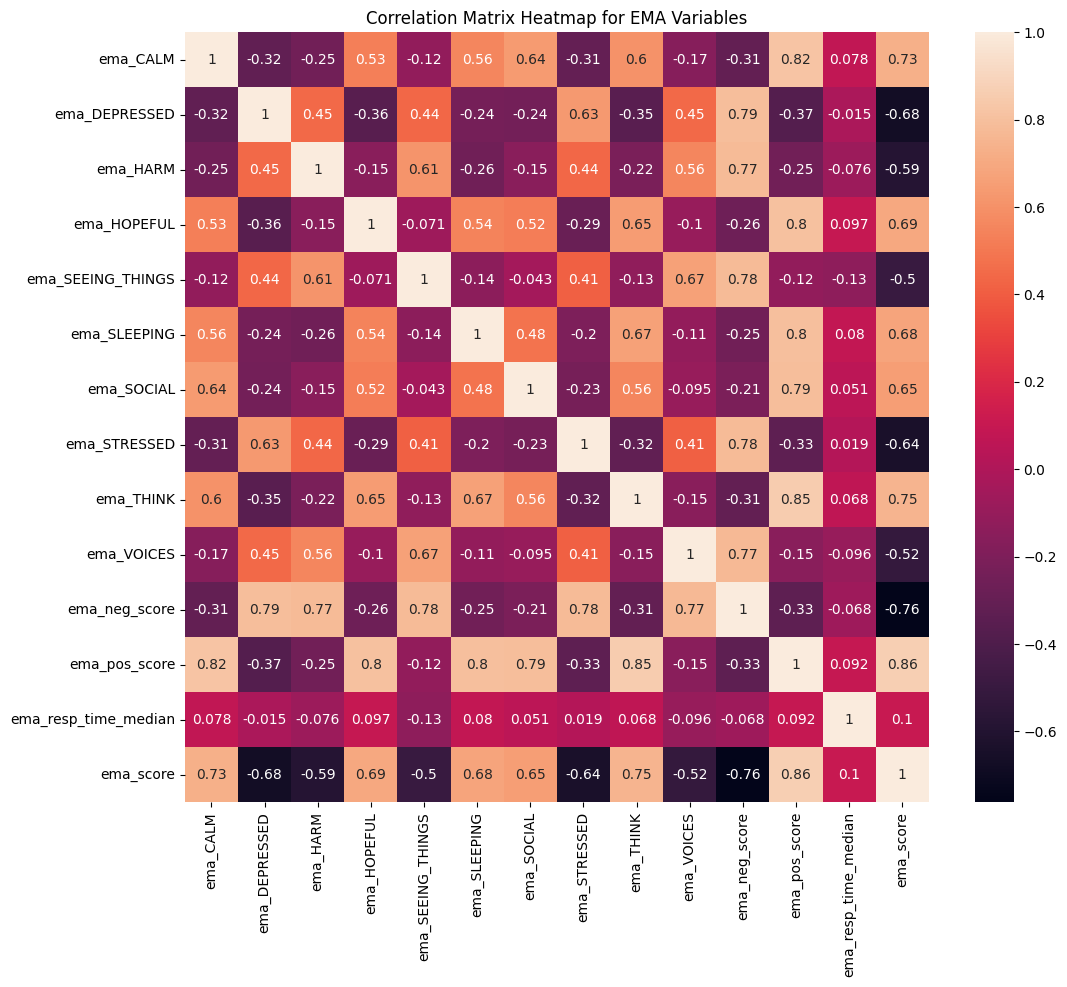
\includegraphics[width=0.5\linewidth]{Dissertation 24/heatmap.png}
    \caption{Correlation Analysis of EMA}
    \label{cor}
\end{figure}
\begin{figure}[H]
    \centering
    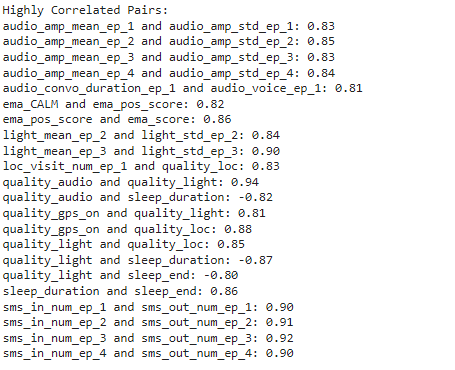
\includegraphics[width=0.5\linewidth]{Dissertation 24/high_correlation.png}
    \caption{Correlation of other features}
    \label{corr}
\end{figure}

Figure \ref{cor} and \ref{corr} illustrate the correlation between the EMA and also highlight significant correlations among other features. The EMA (positive, negative, and score) demonstrates a strong positive and negative correlation across all target variables. Specifically, EMA\_positive correlates highly with positive symptoms, while EMA\_negative correlates strongly with negative symptoms. These columns were dropped as they are aggregated results of the various positive and negative scores.
Due to the high degree of multicollinearity generally within the dataset as shown in \ref{corr}, feature selection is essential and this observation further justifies the application of the LassoCV models, which is well-suited for addressing multicollinearity and improving model performance.
\subsubsection{Outlier Detection}




\begin{figure}[H]
    \centering
    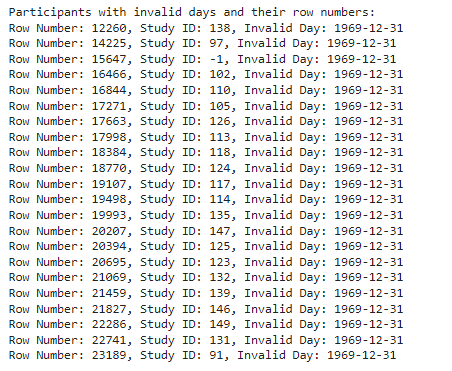
\includegraphics[width=0.5\linewidth]{Dissertation 24/correlation.png}
    \caption{Identified Outlier}
    \label{outler2}
\end{figure}
Using the z-score, a total of 10,002 outliers were detected. The z-score method was chosen because it standardizes the data, making it easier to identify significant deviations, which is crucial in health-related datasets. While these outliers will not be removed as they may represent important clinical variations, an exception is made for an outlier in the "day" column, where the year is recorded as 1969 as shown in Figure \ref{outler2}. This outlier was removed, as the dataset only covers the years 2015 to 2017.

\subsubsection{Missing values and Mismatched Aggregate Score}

\begin{figure}[H]
    \centering
    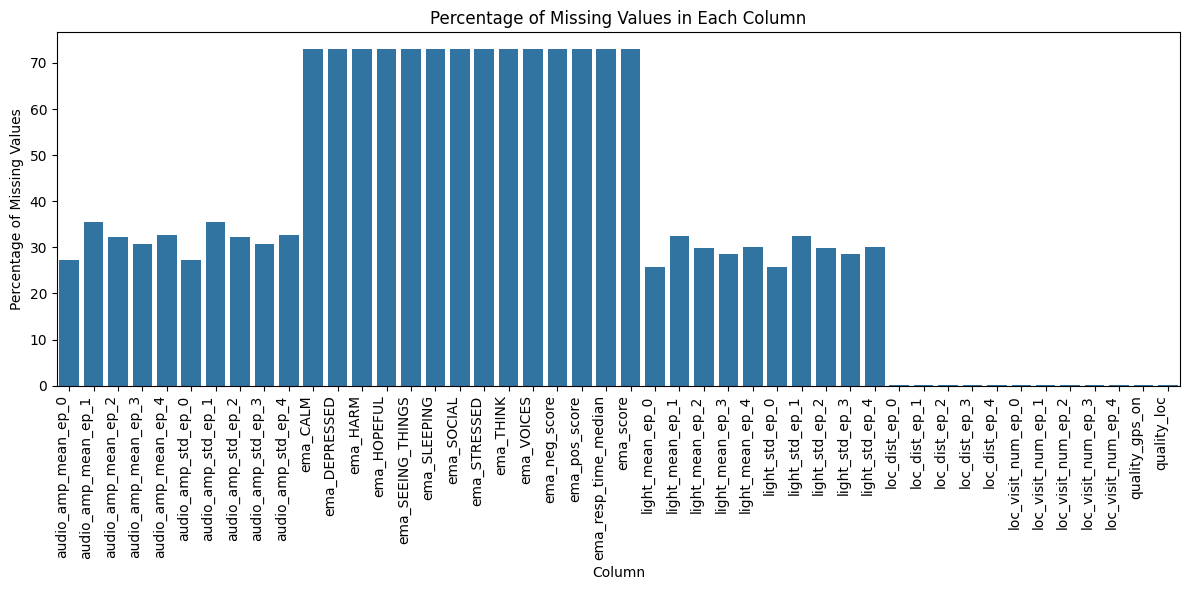
\includegraphics[width=0.5\linewidth]{Dissertation 24/missing values.png}
    \caption{Missing Value Percentage}
    \label{miss}
\end{figure}


\begin{figure}[H]
    \centering
    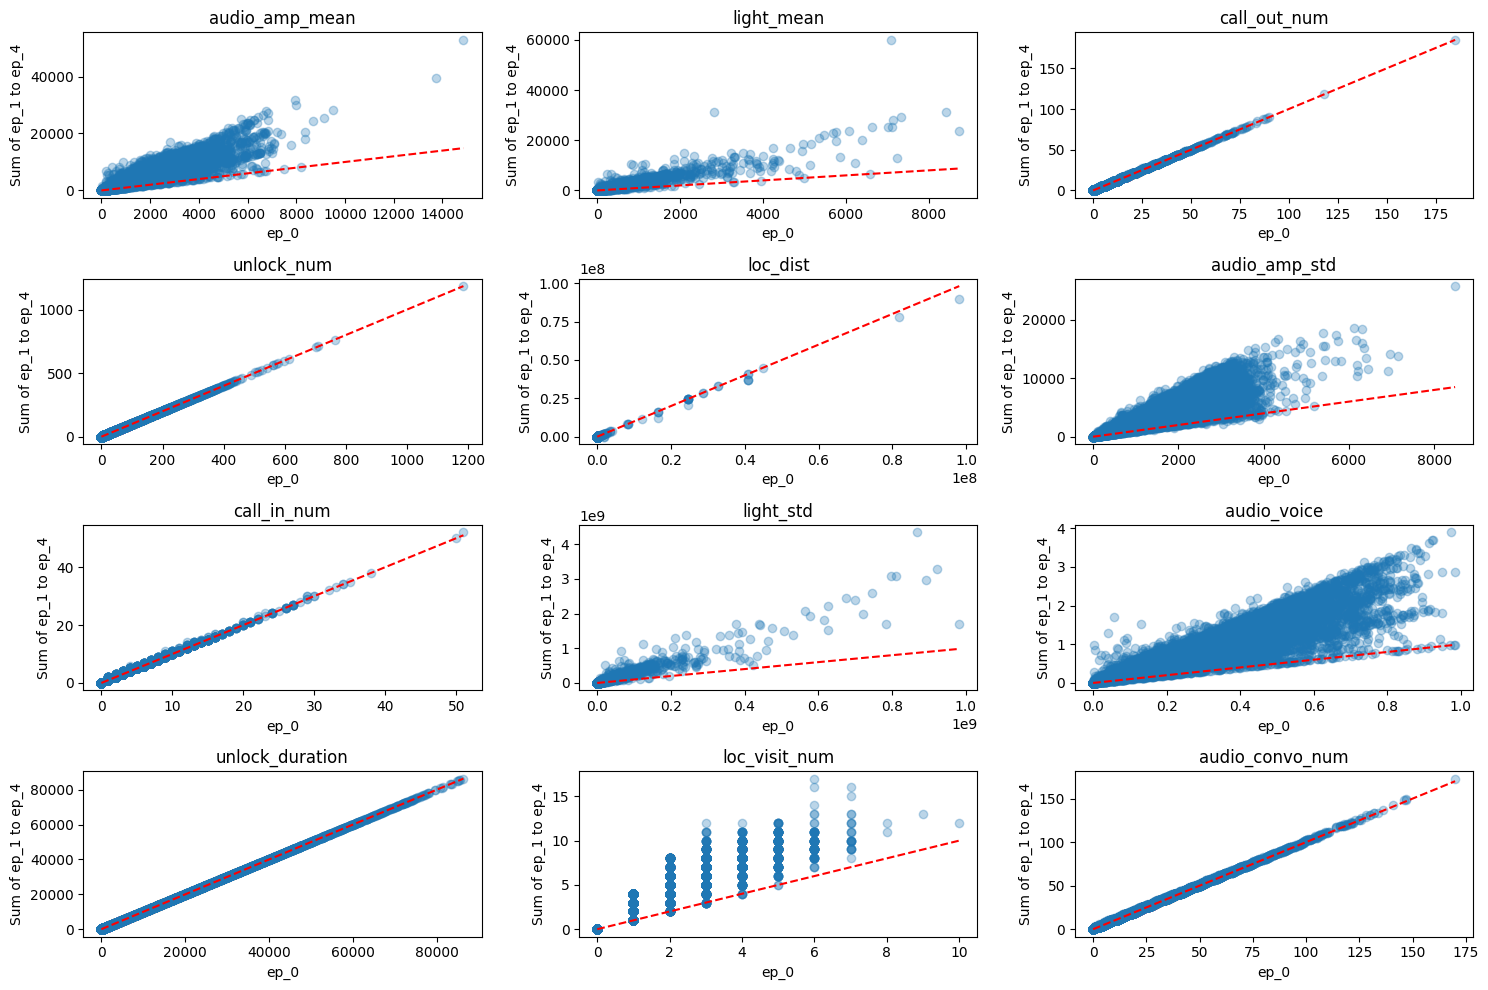
\includegraphics[width=0.5\linewidth]{Dissertation 24/ep_0.png}
    \caption{Aggregated Score for Epoch_0}
    \label{aggr}
\end{figure}

 Figure \ref{miss} illustrates the percentage of the missing data in the datasets while the scatter plots as shown in figure \ref{aggr} visualize the differences among the values in epoch 0 (ep\_0) and the sum of epoch 1-4 for each selected column.The discrepancies between the aggregated episode values and the reported totals (ep\_0) raise concerns about the reliability of the data. Since the summed values do not consistently align with ep\_0, it suggests potential data integrity issues that could negatively impact the analysis or modeling process, the columns were dropped to help avoid potential biases that could skew the results.

\section{Experimental Results}


\subsection{Evaluation of Results For Generalized Model }

\subsubsection{Evaluation of 5 Positive }


\begin{table}[H]
\centering
\caption{RMSE\_STL\_POST\_ and RMSE\_MTL\_POST\_ WITH TUNING}
\label{table:rmse_post_comp_tune}
\begin{tabular}{|l|c|c|}
\hline
\textbf{SYMPTOM} & \textbf{RMSE\_STL\_POST\_} & \textbf{RMSE\_MTL\_POST\_} \\ \hline
CALM & 0.9440423186838058 & 0.9437969762205503 \\ \hline
HOPEFUL & 0.9801633765713665 & 0.9787655753442269 \\ \hline
SLEEPING & 0.9335335511267163 & 0.9326096037267695 \\ \hline
SOCIAL & 0.9542377679345595 & 0.951665717565537 \\ \hline
THINK & 0.9077647518533615 & 0.9073883664439428 \\ \hline
\end{tabular}
\end{table}


\begin{table}[H]
\centering
\caption{RMSE\_STL\_POST and RMSE\_MTL\_POST AUTOMATIC }
\label{table:rmse_post_compP_auto}
\begin{tabular}{|l|c|c|}
\hline
\textbf{SYMPTOM} & \textbf{RMSE\_STL\_POST} & \textbf{RMSE\_MTL\_POST} \\ \hline
CALM & 0.9440290814743473 & 0.9440282511137151 \\ \hline
HOPEFUL & 0.9801637416300867 & 0.9788070117579115 \\ \hline
SLEEPING & 0.9337375219713796 & 0.9327292322207583 \\ \hline
SOCIAL & 0.953966732943221 & 0.9518563150050731 \\ \hline
THINK & 0.9076004187270317 & 0.9074626012701574 \\ \hline
\end{tabular}
\end{table}



Table \ref{table:rmse_post_comp_tune} and \ref{table:rmse_post_compP_auto} displays the result of the RMSE values for positive symptoms (ema\_CALM, ema\_HOPEFUL, ema\_SLEEPING, ema\_SOCIAL, and ema\_THINK) using automatic selection and hyperparameter tuning approach. The RMSE values across symptoms suggest comparable performance between the MTL and STL models, indicating that the models’ inbuilt structures are fairly robust even without parameter fine-tuning. However, notable observations include slightly higher RMSE values for symptoms like ema\_HOPEFUL and ema\_SOCIAL, suggesting these symptoms are inherently more challenging to predict accurately without hyperparameter tuning.
For hyperparameter tuning, the RMSE values for MTL and STL show slight improvements across all symptoms, indicating that hyperparameter tuning effectively reduces the prediction error and enhances model accuracy.
A notable improvement can be seen particularly in the symptoms where automatic selection had higher RMSE values (ema\_HOPEFUL and ema\_SOCIAL), suggesting that tuning helps the models better capture the complexities associated with these symptoms.

Overall, it can be observed that MTL in ema\_SOCIAL significantly outperforms STL, demonstrating a clear benefit in predicting social engagement, likely due to MTL’s ability to generalize better by learning from related tasks.

\subsubsection{Evaluation of 5 Negative}

\begin{table}[H]
\centering
\caption{ RMSE\_STL\_NEGT and RMSE\_MTL\_NEGT AUTOMATIC SELECTION}
\label{table:rmse_negt_comparison}
\begin{tabular}{|l|c|c|}
\hline
\textbf{SYMPTOM} & \textbf{RMSE\_STL\_NEGT} & \textbf{RMSE\_MTL\_NEGT} \\ \hline
DEPRESSED & 0.8707861943261692 & 0.8709503395531324 \\ \hline
HARM & 0.7338423144323089 & 0.7338896618167826 \\ \hline
SEEING\_THINGS & 0.6621302827920619 & 0.6615085027316516 \\ \hline
STRESSED & 0.9082293785796758 & 0.9086949315186562 \\ \hline
VOICES & 0.7126534555866278 & 0.7118239120291409 \\ \hline
\end{tabular}
\end{table}


\begin{table}[H]
\centering
\caption{RMSE\_STL\_NEGT\_ and RMSE\_MTL\_NEGT\_ WITH TUNING}
\label{table:rmse_negt_compar_tune}
\begin{tabular}{|l|c|c|}
\hline
\textbf{SYMPTOM} & \textbf{RMSE\_STL\_NEGT\_} & \textbf{RMSE\_MTL\_NEGT\_} \\ \hline
DEPRESSED & 0.8707344204016165 & 0.8709455386958265 \\ \hline
HARM & 0.7338139099483555 & 0.7338700283664642 \\ \hline
SEEING\_THINGS & 0.6621647753710903 & 0.6614979596820757 \\ \hline
STRESSED & 0.9082427284154707 & 0.9087051087700354 \\ \hline
VOICES & 0.7126834255749256 & 0.7118139741107232 \\ \hline
\end{tabular}
\end{table}





From Table \ref{table:rmse_post_comp_tune} and \ref{table:rmse_negt_comparison}, it can be observed that highest RMSE values are observed for ema\_DEPRESSED and ema\_STRESSED, suggesting these symptoms are the most challenging to predict accurately without any specific tuning of model parameters. In addition, ema\_HARM and ema\_VOICES exhibit relatively lower RMSE values, while ema\_VOICES exhibit the lowest RMSE, indicating better prediction accuracy for these symptoms using automatic selection settings. Noticeable improvement in RMSE is observed across most negative symptoms, highlighting the impact of hyperparameter optimization. However, the reduction in RMSE is most evident for ema\_DEPRESSED and ema\_STRESSED, showing that tuning allows the models to better capture the nuances of these more complex symptoms.

\subsubsection{Evaluation of the 10 symtpoms}


\begin{table}[H]
\centering
\caption { RMSE\_STL\_ALL and RMSE\_MTL\_ALL AUTOSELECTION}
\label{table:rmse_all_auto}
\begin{tabular}{|l|c|c|}
\hline
\textbf{SYMPTOM} & \textbf{RMSE\_STL\_ALL} & \textbf{RMSE\_MTL\_ALL} \\ \hline
CALM & 0.9440290814743473 & 0.9435889162878031 \\ \hline
DEPRESSED & 0.8707861943261692 & 0.8698068586912407 \\ \hline
HARM & 0.7338423144323089 & 0.732622146160298 \\ \hline
HOPEFUL & 0.9801637416300867 & 0.978839169036284 \\ \hline
SEEING-THINGS & 0.6621302827920619 & 0.6600505082846763 \\ \hline
SLEEPING & 0.9337375219713796 & 0.9327071767210345 \\ \hline
SOCIAL & 0.953966732943221 & 0.9514929888502515 \\ \hline
STRESSED & 0.9082293785796758 & 0.9085697250831047 \\ \hline
THINK & 0.9076004187270317 & 0.9074609724703986 \\ \hline
VOICES & 0.7126534555866278 & 0.7110974444954095 \\ \hline
\end{tabular}
\end{table}

\begin{table}[H]
\centering
\caption{ RMSE\_STL\_ALL\_ and RMSE\_MTL\_ALL\_ WITH HYPERPRARAMETER TUNING}
\label{table:rmse_all_hyper}
\begin{tabular}{|l|c|c|}
\hline
\textbf{SYMPTOM} & \textbf{RMSE\_STL\_ALL\_} & \textbf{RMSE\_MTL\_ALL\_} \\ \hline
CALM & 0.9440423186838058 & 0.9434783323311083 \\ \hline
DEPRESSED & 0.8707344204016165 & 0.869867813851116 \\ \hline
HARM & 0.7338139099483555 & 0.7327300821794693 \\ \hline
HOPEFUL & 0.9801633765713665 & 0.9788254402549237 \\ \hline
SEEING-THINGS & 0.6621647753710903 & 0.6601148724496688 \\ \hline
SLEEPING & 0.9335335511267163 & 0.9326533467370749 \\ \hline
SOCIAL & 0.9542377679345595 & 0.9513992752677108 \\ \hline
STRESSED & 0.9082427284154707 & 0.9085005571160768 \\ \hline
THINK & 0.9077647518533615 & 0.9074351810213355 \\ \hline
VOICES & 0.7126834255749256 & 0.711142795005065 \\ \hline
\end{tabular}
\end{table}







For most symptoms, the RMSE values the MTL outperforms the STL However, for ema\_STRESSED, STL performs slightly better than MTL, highlighting that in some cases, single-task learning might handle the noise and task-specific features better as shown in Table \ref{table:rmse_all_auto} and \ref{table:rmse_all_hyper}

Hyperparameter tuning revealed slightly reduced RMSE for most symptoms, indicating a fine-tuned model can capture more precise patterns in the data,  especially in symptoms like ema\_SOCIAL. Based on the analysis, it is evident that the negative symptoms—specifically ema\_SEEING-THINGS, ema\_VOICES, and ema\_HARM—consistently demonstrate lower RMSE values compared to the positive symptoms. This suggests that the negative symptoms are predicted with greater accuracy and stability within the model. The lower RMSE values indicate a closer alignment between predicted and actual observations, highlighting the model's effectiveness in capturing the nuances associated with negative symptoms, while the positive symptoms appear to present more variability or complexity in prediction. To determine whether the observed differences in STL and MTL are statistically significant, the Wilcoxon signed-rank test was employed. 



\subsubsection{Statistical Analysis}


\begin{table}[H]
\centering
\caption{Wilcoxon Test Results With Automatic Selection}
\label{tab:wilcoxon_test_results}
\begin{tabular}{|l|c|c|c|}
\hline
\multicolumn{4}{|c|}{\textbf{WILCOXON TEST RESULTS}} \\ \hline
\textbf{SYMPTOM} & \textbf{NEGATIVE} & \textbf{POSITIVE} & \textbf{ALL} \\ \hline
P-VALUE & 0.8125 & 0.0625 & 0.005859 \\ \hline
\end{tabular}
\end{table}

\subsubsection{HYPERPARAMETER TUNING}

\begin{table}[H]
\centering
\caption{Wilcoxon Test Results With Hyperparameter Tuning}
\label{tab:wilcoxon_test_hyper}
\begin{tabular}{|l|c|c|c|}
\hline
\multicolumn{4}{|c|}{\textbf{WILCOXON TEST RESULTS}} \\ \hline
\textbf{SYMPTOM} & \textbf{NEGATIVE} & \textbf{POSITIVE} & \textbf{ALL} \\ \hline
P-VALUE & 0.8125 & 0.0625 & 0.00390625 \\ \hline
\end{tabular}
\end{table}

The results, presented in Tables \ref{tab:wilcoxon_test_results} and \ref{tab:wilcoxon_test_hyper}, demonstrate that MTL shows statistically significant improvements across when all the 10 symptoms: CALM, DEPRESSED, HARM, HOPEFUL, SEEING\_THINGS, SLEEPING, SOCIAL, STRESSED, THINK, and VOICES were employed. With hyperparameter tuning, MTL achieved a p-value of 0.0039, outperforming the automatic selection approach, which yielded a p-value of 0.0059. This underscores the enhanced efficacy of MTL when tailored to the specific characteristics of the tasks involved.


 







\subsection{Personalized Model Analysis}
. 
\begin{figure} [H]
    \centering
    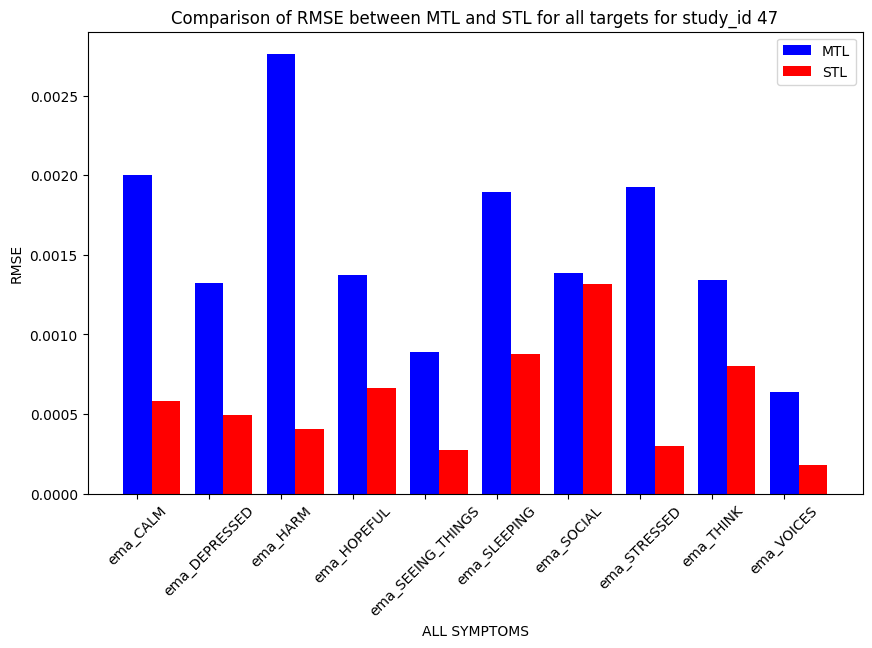
\includegraphics[width=0.5\linewidth]{RMSE_ALL_AUTO_47.png}
    \caption{RMSE FOR STL AND MTL\_ALL FOR STUDY ID 47}
    \label{RMSE_ALL_47}
\end{figure}

\begin{figure}[H]
    \centering
    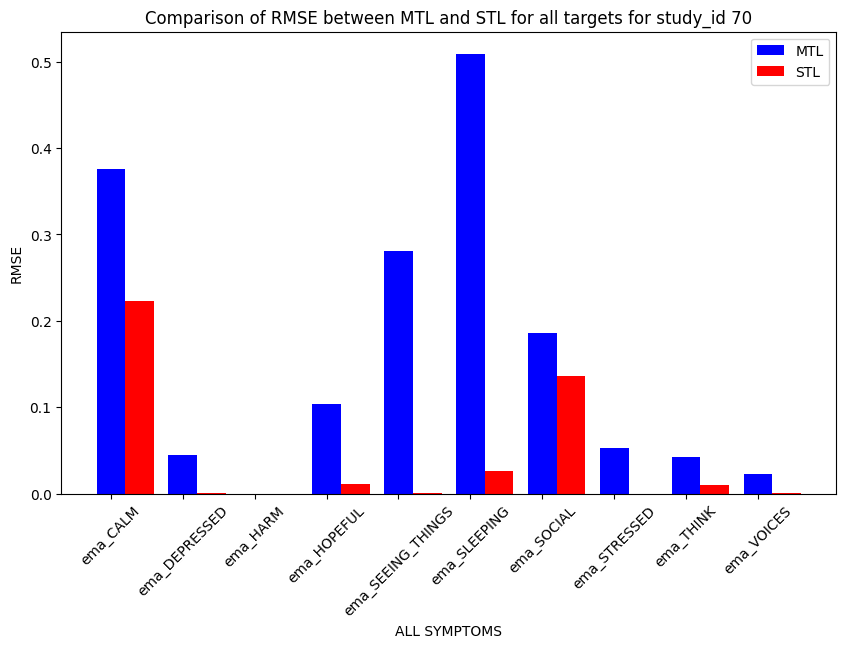
\includegraphics[width=0.5\linewidth]{RMSE_ALL_AUTO_70.png}
    \caption{RMSE FOR STL AND MTL\_ALL FOR STUDY ID 70}
    \label{RMSE_ALL_70}
\end{figure}

Based on the results presented in Figures \ref{RMSE_ALL_47} and \ref{RMSE_ALL_70}, it is evident that Single Task Learning (STL) consistently outperforms Multitask Learning (MTL) across both studies, with Study\_id 47 comprising 408 entries and Study\_id 70 containing 22 entries. The consistently higher RMSE values observed in MTL highlight the potential challenges inherent in multitasking learning, likely due to inadequate or insufficiently distinct shared features for modeling as opposed to the amount to features examined by \citet{tseng2020using}.The smaller dataset size, particularly in Study\_id 70, exacerbates this issue, as MTL depends on sufficient data to effectively learn shared representations across tasks. With limited data, MTL's ability to identify meaningful shared features diminishes, making it more difficult to model individual tasks accurately. This data scarcity can lead to suboptimal shared representations, failing to capture the critical task-specific nuances and resulting in poorer overall performance compared to STL.The statistical significance of these findings is underscored by the p-value of 0.008, indicating a highly significant difference in performance between STL and MTL. This p-value confirms that the observed performance advantage of STL over MTL is not due to random chance, further validating the superiority of task-specific learning models, especially in scenarios with smaller datasets where MTL's shared feature approach is particularly challenged. 

The overall comparative analysis of MTL and STL for all methodologies except the personalized indicates that MTL generally exhibits superior performance than STL, especially when hyperparameters are fine-tuned. This advantage stems from MTL’s ability to leverage inter-task correlations, enhancing its predictive accuracy.




\section{Comparison Against Other Studies}
This study presents a novel approach in comparing single-task learning (STL) and multitask learning (MTL) using a consistent algorithmic framework, specifically LassoCV for STL and its variant MultiTaskLassoCV for MTL. In contrast, \citet{tseng2020using} explored a broader range of algorithms to evaluate both STL and MTL, highlighting that while MTL generally outperformed STL in both generalized and personalized models, only the difference in personalized performance was statistically significant. This divergence underscores the value of comparing STL and MTL within a unified model framework, as seen in the current study, which helps provide a clearer evaluation of model performance by using common evaluation criteria.

Another critical distinction between the studies is the difference in dataset size and feature complexity. While \citet{tseng2020using} utilized 4,157 original features in their analysis, this study examined only 155 features. This stark difference in feature space directly influences the models' capability to capture complex relationships within the data. The impact of this is particularly evident when comparing personalized MTL and STL models, where a higher feature count allows for more nuanced and detailed personalization. The smaller feature set in this study likely constrained the model's ability to fully leverage the personalized advantages of MTL, providing a compelling point of contrast against the findings of \citet{tseng2020using}.

This study’s approach of using the same base algorithm with STL and MTL variants contributes to the literature by providing insights into the performance of models under uniform evaluation conditions, thus avoiding the confounding effects of algorithmic diversity seen in previous studies. This methodological consistency facilitates a more precise understanding of the inherent strengths and limitations of STL and MTL approaches when applied to similar tasks.


\section{Limitations and Scope for Improvement}
\subsection{Limitations}

A primary limitation of this study arises from the dataset size and quality. The relatively small dataset used in this study, coupled with the substantial amount of missing data, poses challenges in achieving robust and personalized results. The limited sample size restricts the statistical power of the findings, and missing data can introduce biases or lead to inaccurate conclusions, especially in personalized models where data sparsity can significantly affect individual predictions.


The computational complexity of the MultiTaskLassoCV model presents another substantial challenge, particularly in the context of personalized modeling with hyperparameter tuning. This approach requires considerable computational resources and extended processing time, especially when handling large-scale or high-dimensional datasets. These demands can become a bottleneck in the model training and optimization process, limiting the scalability and practical applicability of this approach to larger or more complex datasets. Additionally, the increased complexity associated with hyperparameter tuning in MTL can result in suboptimal model performance if not meticulously managed, further complicating the balance between model complexity and computational feasibility.



Another significant limitation is the selection of LassoCV as the model for both STL and MTL comparisons. While LassoCV excels at feature selection and regression through the integration of regularization with cross-validation, it is not specifically tailored for sequential data or temporal machine learning tasks. The application of LassoCV to a time-series dataset limits its effectiveness, as it lacks mechanisms to capture temporal dependencies inherent in sequential data. Models such as Recurrent Neural Networks (RNNs) or Temporal Convolutional Networks (TCNs), which are designed to handle the temporal nature of data, could potentially offer superior predictive performance and interpretability by leveraging these time-dependent relationships.



\subsection{Scope for Improvement}

To enhance the effectiveness of the approach, future research could explore the integration of models specifically designed for time-series analysis, such as Recurrent Neural Network (RNN) or Temporal Convolutional Networks (TCNs). These models can better capture temporal dependencies and might improve the accuracy and interpretability of predictions, particularly for datasets with sequential characteristics. Moreover, expanding the dataset size and improving data quality could help improve model performance and the reliability of results.

To mitigate the computational complexity associated with MultitaskLassoCV, alternative approaches such as dimensionality reduction techniques (e.g., Principal Component Analysis, PCA) could be employed before model training. Additionally, leveraging parallel processing or cloud computing resources might help in managing the computational demands, allowing for more efficient model training and evaluation.



\def\baselinestretch{1.44}

%%% ----------------------------------------------------------------------


   
\smallskip
%%% ----------------------------------------------------------------------
\goodbreak








\def\baselinestretch{1.66}
\medskip

%%% ----------------------------------------------------------------------
